

\documentclass[12pt, a4paper, titlepage]{article}

\usepackage{mathtools}
\usepackage{amssymb}
\usepackage{amsthm}
\usepackage{amsmath}
\usepackage{pdfpages}

\newtheorem{proposition}{Proposition}
\newtheorem{lemma}{Lemma}
\newtheorem{definition}{Definition}
\newtheorem{corollary}{Corollary}
\newtheorem{remark}{Remark}
\newtheorem{thm}{Theorem}

\begin{document}



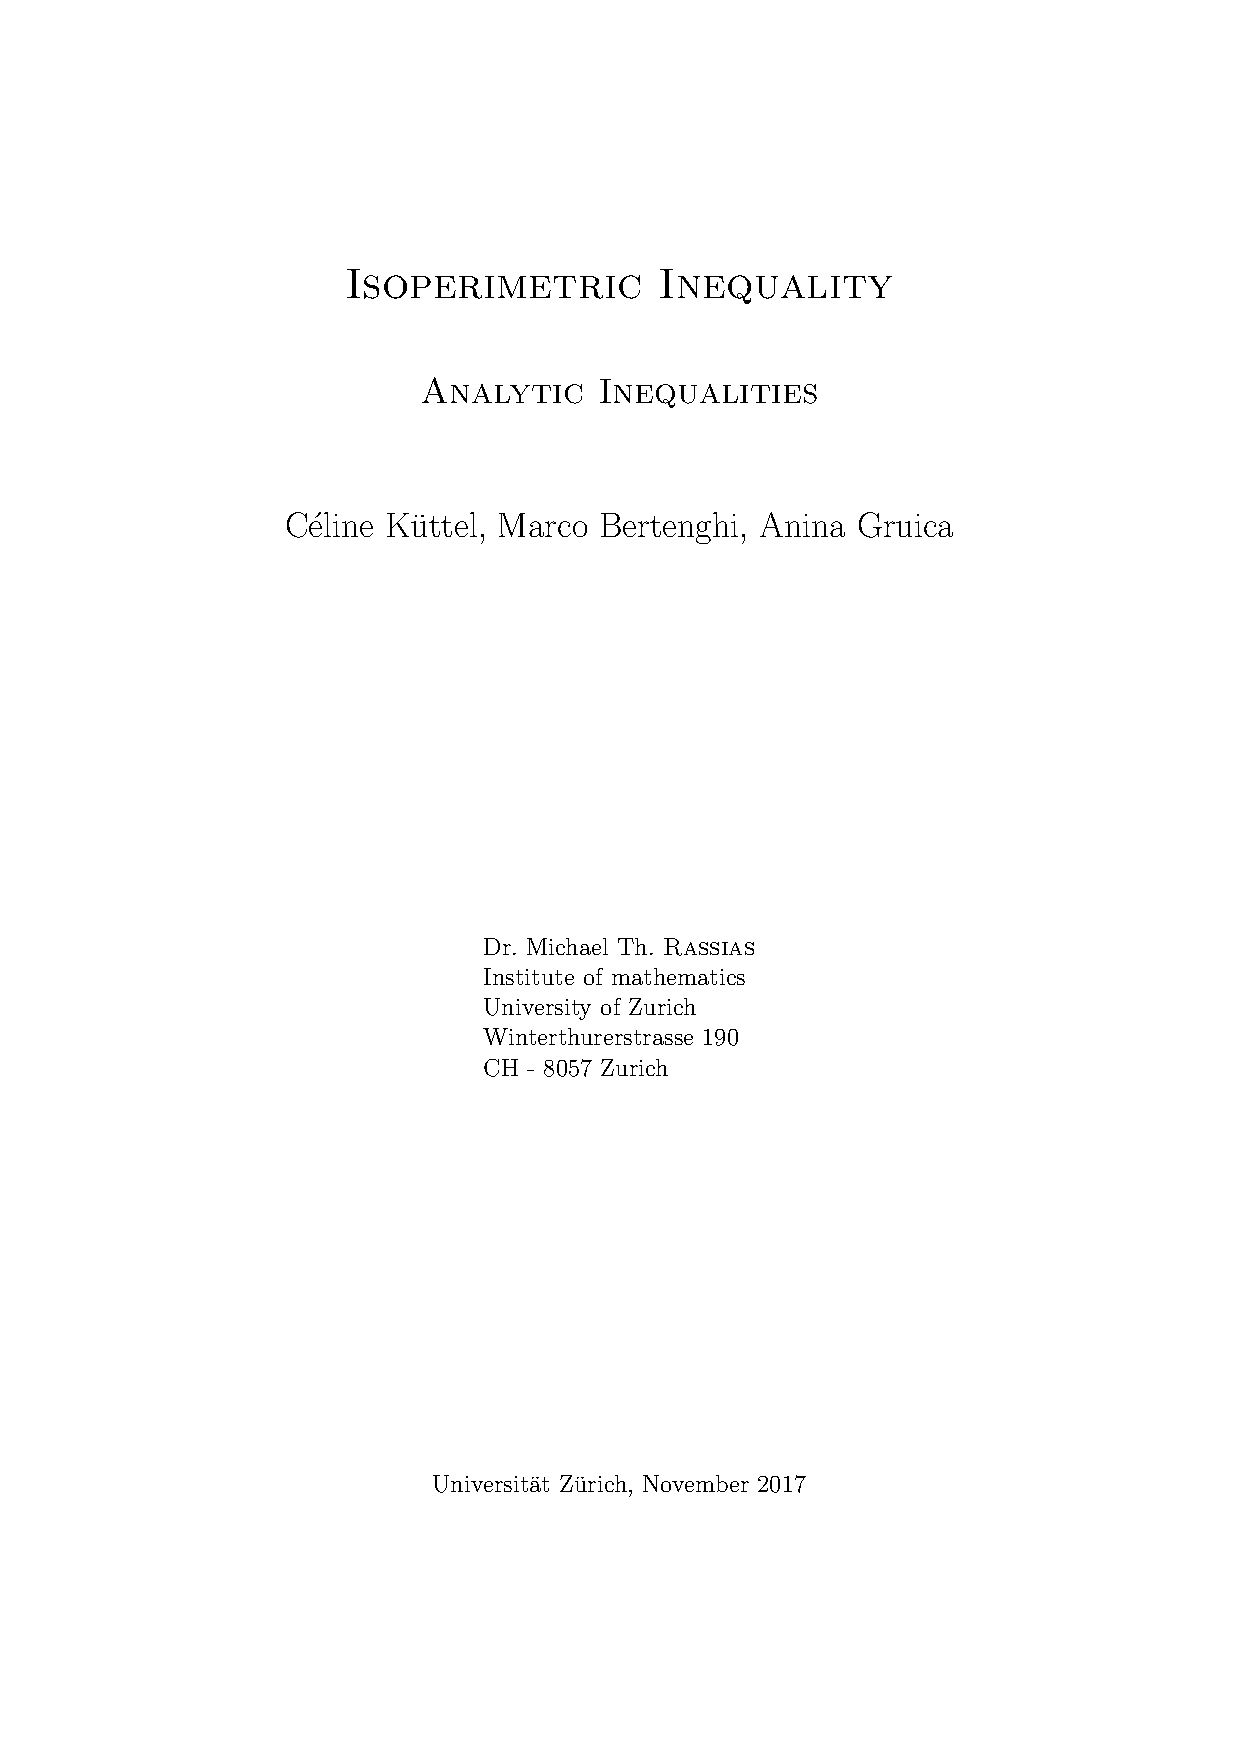
\includepdf{titlePage}
\textbf{Abstract:} We present a self-contained discussion of the classical isoperimetric problem. In the first section, we briefly take a glance at its place in history and evolution thorough, up until more recent developments in mathematics such as optimal transport. The second section gives a complete proof of the planar isoperimetric inequality by Hurwitz. Finally, in the last section, we present a proof by induction over the dimension $n$ to obtain a generalised version of the isopermetric inequality.
\tableofcontents 
\newpage


%%%%%%%%%%%%%%%%%%%% BEGIN CELINES PART %%%%%%%%%%%%%%%%%%%

\section{Formulation of the theorem}
\begin{thm}[The Isoperimetric Inequality]
Let $c(t)=(x(t),y(t))$ be a simple, closed, positively oriented and regular parameterised $C^1$ curve with t $\in$ $[a,b]$. Denote the area enclosed in the above defined curve c(t) with A. \\
For a given length l of c(t)=(x(t),y(t)), we then have
\begin{align*}
4 \pi A \leq l^2,
\end{align*}
with equality iff c(t) is a circle.

\end{thm}
\section{History}
To emphasize the significance of the isomorphic inequality, we will start with its history which dates back to antique literature and geometry, giving physical insight into nature phenomena as well. %%% Isoperimetric inequality DOES NOT answer why Bee's build hexagonal shapes.
\subsection{The legend of Dido}
Historically the problem can be dated back to Vergil's Aenid and his tale of the foundation of the city Carthage.
\begin{verse}
At last they landed, where from far your eyes,\\
May view the turrets of new Carthage rise;\\
There bought a space of ground, which Byrsa call'd,\\
From the bull's hide they first inclos'd, and wall'd.
\end{verse}

Vergil's version has it that Queen Dido from Phoenicia, daughter of the king of Tyre fled her home after her bloodthirsty brother had killed her husband. She ended up on the north coast of Africa where she made a deal with a local chieftain: In return for her fortune she could get as much land as she could enclose with an oxhide. Dido cut the hide into very thin strips, tied them together and constructed a huge semicircle which together with the natural boundary of the sea, turned out to be bigger than anyone could have imagined. Upon this land, Carthage was established.\\\\
It seems as if Dido knew the isoperimetric inequality and understood how to apply it to get the best possible solution. 
This was essential for the mathematics as well as the progress of the story. Vergil tells us that Aeneas, on his quest to found Rome, was shipwrecked and blown ashore at Carthage. Dido fell in love with him but he did not return her love so he sailed away and Dido killed herself. So it was concluded that such an ungrateful and unreceptive man caused the loss of a potential mathematician.
\subsection{Connection to modern mathematics: optimal transportation}
As with circles and the maximal area, we have the same question in three dimensions: Given a certain volume, what is the least surface area needed to enclose it? The answer is given to us by soap bubbles: the sphere. The bubble adjusts its shape to minimize its energy tension, given a certain amount of air.
This can be generalized. Crystals for example take a certain shape that have the least surface energy at fixed volume. But what happens when you add more energy?\\
\\
Alessia Figalli took inspiration in that problem. He applied methods of a modern branch of mathematics, known as optimal transport, in order to understand how individual particles move along the process of heating the crystal, to then understand the change in shapes. His research culminated in the following theorem, for which he was awarded with a fields medal in 2018:
\begin{thm}[Figalli, Maggi, Pratelli]
The shape of the crystal can change at most by $\sqrt{\epsilon}$, where $\epsilon$ is the amount of energy added to the system.

\end{thm}

\subsection{First geometric proofs}
The history of geometric proofs goes back to the ancient Greeks. The Greeks pretty much solved it, by their standards, when Zenodorus proved that a circle has a greater area than any polygon with the same perimeter, but his work unfortunately was lost. We now know it mainly through Pappus and Theon of Alexandria. Pappus' introduction to the subject, in his \textit{Collection}, Book V, is considered a literary masterpiece. In his introduction he tells us about his fascination with bees and how they know that they have to build hexagons.\\\\
Apart from the fascination with bees, motivation for the isoperimetric problem came from astronomy.
According to modern standards, however, the proofs of the ancient Greeks were incomplete since, they apparently did not study the irregular cases. 
\newpage
\subsection{Proofs by Steiner}
In modern days Steiner realized that the Greek arguments were incomplete and established a better way to proof the inequality. \\
It's said that Steiner gave five proofs of the isoperimetric theorem. Three of them will be presented in this paper. Unfortunately all of them had one problem im common: all proofs assume the existence of a solution. His strategy is always to take a figure that is not a circleand show that its area can be improved. But we will see that there are good reasons for considering Steiner's proofs to be essentially complete after all.
\begin{thm}
Any figure with maximal area must be a circle.
\end{thm}
\subsubsection*{Steiner's four-hinge proof}

\begin{proof}
Take a figure with maximal area. Cut its perimeter in half with a line. This line will split thee area in half as well, because if it didn't we could take the half with the greater area together with its reflection in the line and get the a figure with thee same perimeter but greater area. (Figure 1).\\
\begin{figure}[h]
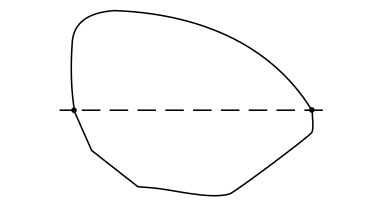
\includegraphics[scale=0.5]{images/Figure1}
\centering
Figure 1
\centering
\end{figure}

Consider one of these halfs. Suppose it is not a semicircle. Then there will be some point on the boundary where lines drawn from the points of on the symmetry line meet at an anfle that is not a right angle Figure 2).\\
\begin{figure}[h]
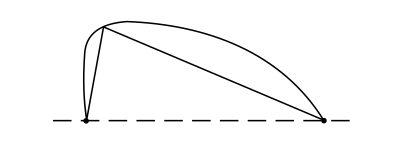
\includegraphics[scale=0.5]{images/Figure2}
\centering
Figure 2
\centering
\end{figure}
\\
Think of there being a void inside the triangle and imagine ths pieces on the sides are glued on. Slide the endpints along the symmetry line to make the angle a right angle(Figure 3).\\
\begin{figure}[h]
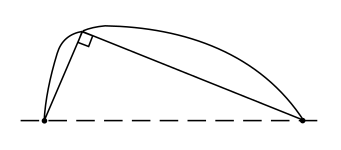
\includegraphics[scale=0.5]{images/Figure3}
\centering
Figure 3
\centering
\end{figure}
\\
This increases the area, so reflecting this ffives a figure with greater area while the perimeter is still the same. That is impossible since we assumed the area to be maximal. So our halves must be semicircles and our figure must have been a circle to start with.
\end{proof}
\begin{remark} \
\begin{enumerate}
\item[a)] If we put the triangles together with their reflection we geet quadrilaterals and we can see the four hinges that have given the proof its name. 
\item[b)] We can use reflection in the midpoint of the symmetry line instead, so that the quadrilaterak becomes a parallelogram. This is slightly more intuitive that straghtening out the parallelogram increases the area.
\end{enumerate}

\end{remark}

\subsubsection*{Steiner's mean boundary proof}

\begin{proof}
Given two curves, consider the mean curve, which is the curve that stays halfway between the tw curves at all times (Figure 4). \\
\begin{figure}[h]
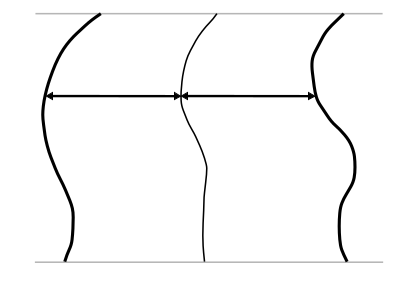
\includegraphics[scale=0.5]{images/Figure4}
\centering
Figure 4
\centering
\end{figure}
\\
The length of this curve will be less than the mean length of the two given curves or qual if thee two curves are the same.. We can see this by slicing the curves into infinitesimals and confirming the claim piecewise.\\
Take a figure with maximal area and cut its perimeter in half with a line (as in Figure 1).\\
As before the line will split the area in half as well, because if it didn't we could take the half with the greater area together with its reflection in the line and get the a figure with thee same perimeter but greater area.\\
Now suppose the two halfs are not reflections of each other. Then reflect them to the same side and draw the mean curve (Figure 5).\\
\begin{figure}[h]
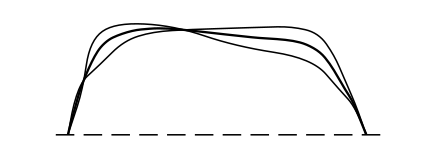
\includegraphics[scale=0.5]{images/Figure5}
\centering
Figure 5
\centering
\end{figure}
\\
This mean curve is shorter but it encloses the same area for it contains all the area that the two curves habe in commom and then hald the addiitonal area of thee firs curve and half the additional area of the second. However, these additional areas are just as large, ensuring ghat the mean curve actually encloses as much as the other curves.\\
So when we cut the perimeter of a maximal figure in half, the halves cannot be different in shape. Otherwise with the construction we just did we would get a figure with the same area but a sammler perimeter. Thus the maximal figure cannot be anything other than a circle.
\end{proof}

\subsubsection*{Steiner's snowball-packing proof}
\begin{proof}
We begin with a convex figure and wish to modify it so that it becomes symmetric in a line. To do this we think of a ficure as consisting of vertical slices, and then we slide each of these slices so that half of each slice lies on eiter side of the line. Firs we consider only polygons. Here we can determine the effect by examining what happens to the vertices: (Figure 6)\\
\begin{figure}[h]
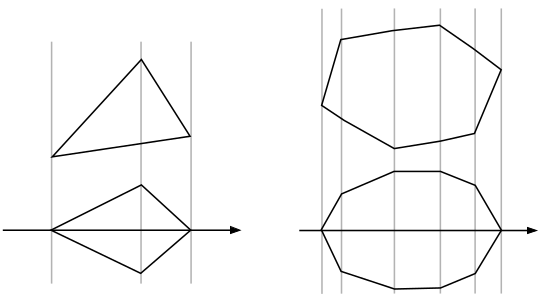
\includegraphics[scale=0.5]{images/Figure6}
\centering
Figure 6
\centering
\end{figure}
\\
The area is still the same but as we see, triangles and trapezoids map to isosceles ones, and these as we know cober area more efficiently.(Figure 7)\\
\begin{figure}[h]
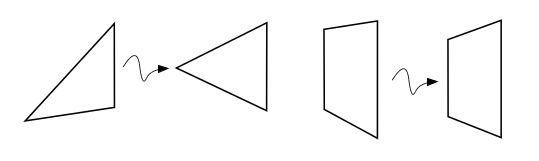
\includegraphics[scale=0.5]{images/Figure7}
\centering
Figure 7
\centering
\end{figure}
\\
For polygons then, the perimeter has decreased unless all triangles and trapezoids are alread isoscles, which occurs when the original figure is symmetric in the line (up to a translation). Applying this to infinitesimals, we are persuaded that the same is true for any convex figure. Thus a solution must be symmetric in every direction, for otherwise we could improve on it. Well this figure must be a circle. Let's look at it a little bit more rigorous:\\
Take such a figure. It will be unaffected (up to transllation) if we make it symmetric in the x-axis and then in the y-axis. But now it must be symmetric in every line through the origin. Surely it mus be a circle. Pedantically consider a point inside the figure and reflect it in all lines through the origin to show that all the other points at the same distance form the origin must also be inside the figure.

\end{proof}

%%%%%%%%%%%%%%%%%%%% END CELINES PART %%%%%%%%%%%%%%%%%%%%%
%%%%%%%%%%%%%%%%%%%% BEGIN ANINAS PART %%%%%%%%%%%%%%%%%%%%

\newpage 
\section{Proof by Hurwitz}
In this section we'll present the proof of the $Isoperimetric$ $Inequality$ that goes back to Hurwitz. He stated the proof in his paper \textit{"Sur le probl\`eme des isop\'erim\`etres"} in 1901. $\\
$First we'll have to state some preliminaries, which we'll later use in the actual proof. The main part of the $Preparation$ $for$ $proof$ $by$ $Hurwitz$ will be $Wirtinger's$ $Inequality$. Using $Wirtinger's$ $Inequality$ we can give a simple proof of the $Isoperimetric$ $Inequality$.

\subsection{Preparation for proof by Hurwitz}

\begin{definition}
A plane curve is a continuous function $\gamma: I \rightarrow \mathbb{R}^2$, $\gamma(t) = (x(t),y(t)) \in \mathbb{R}^2$ where $I$ is an open interval in $\mathbb{R}$ and $x$, $y$ are continuous functions in $\mathbb{R}$. 
\end{definition}

$\\
$

\begin{figure}[htbp] 
  \centering
     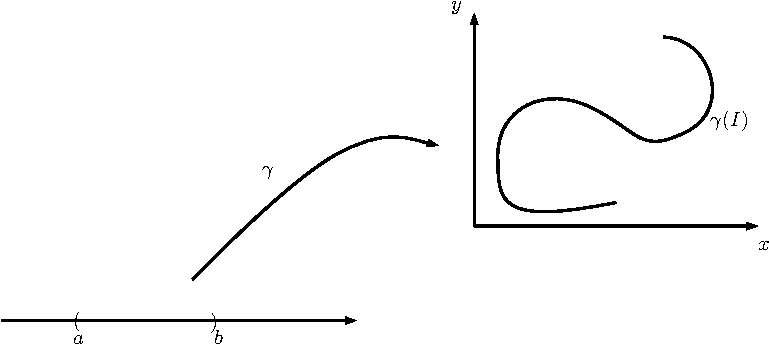
\includegraphics[width=0.8\textwidth]{images/curve.pdf}
  \caption{plane curve}
  \label{fig:Bild2}
\end{figure}

$\\
$

We'll now state some basic but crucial definitions concerning plane curves.

\begin{definition}
Let $\gamma$ be a plane curve on $I=(a,b)$ defined by $\gamma(t) = (x(t),y(t)) \in \mathbb{R}^2$. Then $\\
$
\begin{enumerate}


\item $\gamma$ is called regular if $\gamma(t) \neq 0$ for all $t \in I. \\
$

\item The $arc$ $length$ of $\gamma$ is defined by
\begin{align*}
\int_{a}^{b}|\gamma'(t)|dt = \int_{a}^{b}|(x'(t),y'(t))|dt =\int_{a}^{b}\sqrt{x'(t)^2+y'(t)^2}dt 
\end{align*}

\item If $\gamma'(t)=1$ for all $t \in I$ then $\gamma$ is called parametrized by arc length.

\item A regular curve $\gamma$ is called closed if
\begin{align*}
\gamma(a) = \gamma(b) \\
\gamma'(a) = \gamma'(b) \\
\gamma''(a) = \gamma''(b) \end{align*} \begin{center}
. \\
. \\ 
. \\
\end{center}
i.e., when $\gamma$ and all its derivatives agree at $a$ and $b$.

\item A closed curve $\gamma$ is called simple if there are no self-intersections, i.e., $\gamma(t_1) = \gamma(t_2)$ implies $t_1 = t_2$ for $t_1,t_2 \in I$. Or equivalently, $\gamma$ is injective.

$\\
$

\begin{figure}[htbp] 
  \centering
     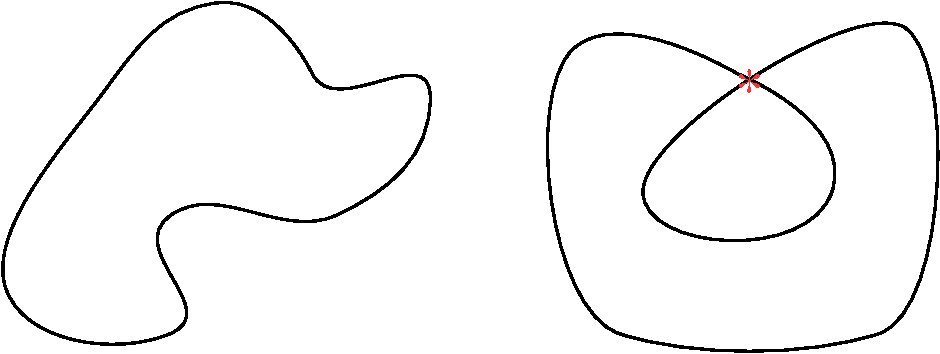
\includegraphics[width=0.8\textwidth]{images/simple.pdf}
  \caption{left: simple curve, right: non-simple curve}
\end{figure}


\item A simple closed curve $\gamma$ is called positively oriented if when travelling on it, one always has the curve interior to the left. 
\end{enumerate}
\end{definition}


\begin{proposition}
Any plane curve can be reparametrized by $arc$ $length$.
\end{proposition}
\begin{proof}
We will proof the following statement: $\\
$
Given $\phi:[a,b] \rightarrow \mathbb{R}^2$ a parametrized curve, we can always find $\psi:[c,d] \rightarrow \mathbb{R}^2$ with $\phi[a,b]=\psi[c,d]$ and $|\psi'(t)|=1$ for all $t \in [c,d]\\
$
The way to prove this is to guess what $\psi$ should be and then find such $\psi$. We know that we should have $\psi = \phi\circ f$ for some increasing function $f$. Hence, with $t=f(s)$ we want that 
\begin{align*}
1 = |\psi'(s)| = f'(s)|\phi'(f(s))| \Rightarrow f'(s)=\frac{1}{|\phi'(f(s))|} = \frac{1}{\phi'(t)|}
\end{align*}
So set $h=\int_a^t|\phi'(u)|du$. then $h'(t)=|\phi'(t)|$ and we choose f to be the inverse of $h$. which much exist and then we have $f'(s)= \frac{1}{|\phi'(f(s))|}$.
\end{proof}

\begin{definition}
Let $\gamma: I \rightarrow \mathbb{R}^2$, $\gamma(t) = (x(t),y(t))$ be a positively oriented, closed, simple plane curve where $I = (a,b)$. Then the area $A$ bounded by $\gamma$ is defined as 
\begin{align*}
A(\gamma) = -\int_a^by(t)x'(t)dt = \int_a^by'(t)x(t)dt
\end{align*}
\begin{remark}
The first equality follows directly from \textit{Green's Theorem}, which goes as follows:
\begin{thm}[Green's Theorem]
Let $\gamma$ be a positively oriented, piecewise smooth, simple closed curve in a plane, and let $D$ be the region bounded by $\gamma$. If $P$ and $Q$ are functions of $(x,y)$ defined on an open region containing $D$ and have continuous partial derivatives there, then
\begin{align*}
\oint_\gamma(Pdx + Qdy) = \int\int_D \left(\frac{\partial Q}{\partial x} - \frac{\partial P}{\partial y}\right)dxdy
\end{align*}
where the path integral is traversed counterclockwise.\end{thm} $\\ 
$
Clearly the area D is equal to 
\begin{align*}
\int\int_D 1dxdy
\end{align*}
which is equal to
\begin{align*}
-\oint_C ydx = -\int_a^by(t)x'(t)dt
\end{align*}
by setting $P = -y$ in $Green's$ $Theorem$.

$\\
$
The second equality follows from the Fundamental Theorem of Integration and Differentiation. Since $\gamma$ is a closed curve, we have that $\gamma(a)=\gamma(b)$:
\begin{align*}
\int_a^by'(t)x(t)dt 
&= \int_a^b(y(t)x(t))'dt - \int_a^by(t)x'(t)dt \\
&= [y(b)x(b)-y(a)x(a)]-\int_a^by(t)x'(t)dt  \\
&= -\int_a^by(t)x'(t)dt
\end{align*}
\end{remark}
\end{definition}

\begin{lemma}[Wirtinger's inequality] Let $f(t)$ be a piecewise smooth, continuous $2\pi$-periodic function with mean value 0, i.e., $\int_{0}^{2\pi}f(t)dt=0$. Then
\begin{align*}
\int_{0}^{2\pi}(f')^2dt \geq \int_{0}^{2\pi}f^2dt,
\end{align*}
with equality if and only if $f(t) = a\cos t + b\sin t$ where $a$ and $b$ are constants.
\end{lemma}

To proof this, we'll start with the weaker version of $Wirtinger's$ $inequality$, which goes as follows:

\begin{lemma}[Wirtinger's inequality - weak version] Let $ f: [0,\pi] \rightarrow \mathbb{R} $ be a smooth function on $(0,\pi)$, such that $\lim_{t\rightarrow 0^+}f'(t)$ and $\lim_{t\rightarrow \pi ^-}f'(t)$ exist. Furthermore, we assume $f(0) = f(\pi) = 0$. Then one has
\begin{align*}
\int_{0}^{\pi}(f')^2dt \geq \int_{0}^{\pi}f^2dt,
\end{align*}
with equality if and only if $f(t) = a\sin t$ where $a$ is a constant.
\end{lemma}

\begin{proof}
To show: $\int_{0}^{\pi}(f')^2-f^2dt \geq 0$.
We can do this by finding a function $\phi$ such that
\begin{align*}
\int_{0}^{\pi}(f')^2-f^2dt = \int_{0}^{\pi}(f'-f\phi)^2dt
\end{align*}
Or equivalently
\begin{align*}
\int_{0}^{\pi}2ff'\phi - f^2(1+\phi^2)dt = 0.
\end{align*}
Integration by parts gives
\begin{align*}
\int_{0}^{\pi}2ff'\phi - f^2(1+\phi^2)dt =  \left.f^2\phi\right|^{\pi}_0 - \int_{0}^{\pi}f^2(\phi'+1+\phi^2)dt = 0.
\end{align*}
So for this to be equal to $0$ we want to solve the differential equation $-\phi' = 1 + \phi^2$, which has solution $\phi(t) = -\tan(t + t_0)$. If we take $t_0 = \pi/2$ then $\phi$ is defined everywhere on the interval $(0,\pi)$. We have 
\begin{align*}
\phi(t) = -\tan(t + \pi/2) = -\frac{\sin(t+\pi/2)}{\cos(t+\pi/2)} = -\frac{\cos(t)}{-\sin(t)} = \frac{\cos t}{\sin t}.
\end{align*}
With L'H\^opital's rule we compute
\begin{align*}
\lim_{t\rightarrow 0^+}\frac{f^2\cos t}{\sin t} = \lim_{t\rightarrow 0^+}\frac{2ff'\cos t - f^2 \sin t}{\cos t} = 0.
\end{align*}
as $\lim_{t\rightarrow 0^+}f'(t)$ exists. Analogously we get $\lim_{t\rightarrow \pi ^-}f^2\phi = 0$. It follows that $\int_{0}^{\pi}2ff'\phi - f^2(1+\phi^2)dt = 0$.
\begin{align*}
\int_{0}^{\pi}(f')^2-f^2dt = \int_{0}^{\pi}\left(f'-f\frac{\cos t}{\sin t}\right)^2 dt \geq 0
\end{align*}
with equality if and only if $f'-f\frac{\cos t}{\sin t} = 0$. The solution to the differential equation $f' = f\frac{\cos t}{\sin t}$ is exactly $f(t) = a\sin t$.
\end{proof}

\begin{proof} $(Wirtinger's$ $inequality)$ To extend the proof to the general case of the $Wirtinger's$ $inequality$ with a $2\pi$-periodic function we need to consider poles. The trick is to observe that $f(t_0) = f(t_0+\pi)$ for some $0 \leq t_0 \leq \pi$, because the function $g(t_0) = f(t) - f(t+\pi)$ has opposite signs for $t = 0$ and $t = \pi$. Let $f(t_0) = f(t_0+\pi) = c$. Now we can apply the previous argument to the function $f(t)-c$ with $\phi(t) = \frac{\cos(t-t_0)}{\sin(t-t_0)}$. The same way as in the proof above we get

\begin{align*}
\int_{0}^{2\pi}(f')^2-(f-c)^2dt - \int_{0}^{2\pi}\left(f'-(f-c)\frac{\cos(t-t_0)}{\sin(t-t_0)}\right)^2dt \\
= \left.(f-c)^2\frac{\cos (t-t_0)}{\sin (t-t_0)}\right|^{2\pi}_0 = 0,
\end{align*}
\begin{align*}
\int_{0}^{2\pi}(f')^2-(f-c)^2dt \geq 0
\end{align*}
with equality if and only if $f(t) - c = a\sin(t-t_0).$
Now we want to get rid of the constant $c$. For this we'll use the assumption $\int_{0}^{2\pi}fdt = 0$, so also $2c\int_{0}^{2\pi}fdt=0$. Therefore
\begin{align*}
\int_{0}^{2\pi}(f')^2-f^2dt\geq 2\pi c^2 \geq 0,
\end{align*}
with equality if and only if $c=0$ and $f(t)=a\sin(t-t_0) = \cos(t_0)\sin(t)-\sin(t_0)\cos(t)$.
\end{proof}


\subsection{Proof}
Now we have all the preliminaries we need in order to proof the $Isoperimetric$ $Inequality$.

\begin{thm}[Isoperimetric Inequality] Let $\gamma: I \rightarrow \mathbb{R}^2$, $\gamma(t) = (x(t),y(t)) \in \mathbb{R}^2$ be a simple closed curve with length $l$ defined on $I=(a,b)$. Let $A$ be the area bounded by $\gamma$. Then
\begin{align*}
l^2 \geq 4\pi A
\end{align*}
with equality if and only if $\gamma$ is a circle.
\end{thm}

\begin{proof}
We can assume that $\gamma$ is parametrized by arc length by Proposition 1. This means $\gamma$ is given by two $l$-periodic functions $x(t),y(t)$ such that
\begin{align*}
x'(t)^2+y'(t)^2 = 1 \text{ for all } t \in I.
\end{align*} 
We can easily convert $\gamma$ to a $2\pi$-periodic function by
\begin{align*}
f(\theta) = x\left(\frac{l\theta}{2\pi}\right), \quad g(\theta)= y\left(\frac{l\theta}{2\pi}\right).
\end{align*}
So we have
\begin{align*}
f'(\theta)^2+g'(\theta)^2 = \frac{l^2}{4\pi^2}.
\end{align*}
By a translation we may assume that $\int_0^{2\pi}f(t)dt = 0$.
Now
\begin{align*}
\frac{l^2}{2\pi} = \int_0^{2\pi}f'(t)^2+g'(t)^2dt = \int_0^{2\pi}|\gamma'(t)|^2dt.
\end{align*}
Now we know that the area $A$ bounded by $\gamma$ is equal to $\int_0^{2\pi}g'(t)f(t)dt$. This gives us 
\begin{align*}
l^2 - 4\pi A 
&= 2\pi\int_0^{2\pi}f'(t)^2+g'(t)^2 - 2g'(t)f(t)dt \\
&= 2\pi\int_0^{2\pi}f'(t)^2 + g'(t)^2 - 2g'(t)f(t) +f(t)^2-f(t)^2dt \\
&= 2\pi\int_0^{2\pi}f'(t)^2-f(t)^2dt + 2\pi\int_0^{2\pi}(g'(t)-f(t))^2dt \geq 0
\end{align*}
where the first integral in the last term is non-negative by $Wirtinger's$ $Inequality$ for the function $f(t)$ , and the integrand of the second integral is non-negative. $\\ \\
$
Equality holds if and only if $f(t)=a\sin(t-t_0)$ and $g' = f$, so $g(t)= -a\cos(t-t_0)+c$. Since $\sqrt{f'(t)^2+g'(t)^2} = \frac{l}{2\pi}$, so $\gamma$ is a circle with centre $(0,c)$ and radius $\frac{l}{2\pi}$.
\end{proof}


%%%%%%%%%%%%%%%%%%%%%%%%% END ANINAS PART %%%%%%%%%%%%%%%%%%%%%%%%%%%%%%%%%%%%

%%%%%%%%%%%%%%%%%%%%%%%%% BEGIN MARCOS PART %%%%%%%%%%%%%%%%%%%%%%%%%%%%%%%%%%

\section{The isoperimetric inequality in $\mathbb{R}^n$}

In this final section we will discuss generalisations of the isoperimetric inequality in higher dimensions, that is we establish a similar result in $\mathbb{R}^n$ for $n \geq 3$ which of course stays compatible with the planar case $n=2$. 
\\\\
Before we tackle the isoperimetric inequality in higher dimensions, let us take a heuristic detour to a related problem. Observations in Physics and Biology tell us that nature strives to be as efficient as possible. For example, when we look at how bees are building their honeycombs, the shape they choose to tile it is the hexagon. Pappus of Alexandria was already fascinated by the honeycombs hexagonal structure, he even declared that bees "possessed a divine sense of symmetry". Jan Brozek (1585-1652) turned Pappus observation into a mathematical conjecture: the hexagon tiles the plane with minimal boundary. Stated another way, the optimal way to cover a large region with shapes of the same area while minimizing the boundary is indeed to make use of the hexagonal structure, as demonstrated by the bees in nature. Thomas Hales finally settled this conjecture in 1998.
\\\\
From the above paragraph we gather that nature sometimes provides elegant and efficient answers to interesting mathematical problems. In fact, in the story discussed above nature dictates us even a candidate (i.e. the hexagon) that solves our problem. This is particularly useful because it allows us to strengthen the conjecture from "there exists an optimal way to tile the plane" to the more satisfactory "there exists an optimal shape to tile the plane with and said shape is a hexagon". It is then the joy of mathematicians to turn those observations into a precise mathematical conjecture and finally prove said conjecture to embed it as a theorem in the world of mathematics. 
\\\\
Let us now return to our goal of studying the isoperimetric problem in higher dimensions. Consider the case $n=3$, because the human eye can perceive $3$-dimensional objects. In light of the isoperimetric inequality, we wonder if nature might again provide us with an insight on most efficient enclosers of volume. Indeed, if we think about soap bubbles in absence of exogenous perturbation or strain, the shape they form is a sphere. 
\\\\
One might take away from this discussion that the isoperimetric inequality is interesting for a multitude of reasons. It is a problem known since ancient Greece, whose solution -apart from being a fundamental mathematical contribution- is both challenging (first proof in 19th century) and beautiful in the sense that it can be motived by phenomena observable in nature.
\newpage 
\begin{thm}[Isoperimetric inequality] \label{T1} Round circles, spheres and hyperspheres are the most efficient enclosers of volume in all dimensions; more precisely, for any domain $K \subset \mathbb{R}^n$ (with sufficiently smooth boundary $\partial K$) with $n$-dimensional volume denoted by $|K|$ and surface area denoted by $| \partial K|$, we have
\begin{align*}
\frac{|K|^{n-1}}{| \partial K|^n} \leq \frac{|B_n|^{n-1}}{| \partial B_n|^n},
\end{align*}
where $B_n$ is the $n$-dimensional sphere and $\partial B_n$ its associated surface. Equality holds if and only if $K$ is a $n$-dimensional sphere.
\end{thm}
For the sake of mathematical completeness we briefly want to discuss some of the pitfalls with the above formulation of the isoperimetric inequality. The quantities on the right hand side of the inequality in theorem \ref{T1} are always well-defined, indeed there are even closed formulas for both $|B_n|$ and $| \partial B_n|$ for all $n \in \mathbb{N}$.
\\
\\
However, on the left hand side of the inequality we need to be a bit more careful when it comes to defining $|K|$ and $| \partial K|$. From measure theory we know that not every subset of $\mathbb{R}^n$ is measurable (in the Lebesgue sense), arguably the most famous counterexample is given by $V \subset \mathbb{R}^n$ where $V$ is the Vitali set. 
\\\\
Hence we insist on $K \subset \mathbb{R}^n$ to be a domain. Recall that  a domain is any connected open subset of a finite-dimensional vector space. Then $|K|:= \lambda_n(K)$ is well-defined where $\lambda_n$ denotes the $n$-dimensional Lebesgue measure. Nevertheless we are not allowed to use the same measure $\lambda_n$ to define $| \partial K|$ because it has a lower dimension than $K$ and hence we have $\lambda_n( \partial K) = 0$, if $\partial K$ is in fact even Lebesgue measurable. Thus we require the topological boundary $\partial K$ of $K$ to be sufficiently smooth in order to make sure we can measure it, again in the Lebesgue sense. Then we can in fact define $| \partial K| := \lambda_{n-1}( \partial K)$. 
\\\\
The aforementioned mathematical arguments become quite technical and involved when we want to be precise. For a more general setting (no additional assumptions on the boundary $\partial K$) we would require the use of Hausdorff measures $\mathcal{H}$ to rigorously define $| \partial K| = \mathcal{H}_{n-1}( \partial K)$. For the sake of simplicity this will be omitted here. 
\\\\
The take away message from this technical detour should be that we want to work in a "sufficiently smooth" setting, such that all quantities that appear in the isoperimetric inequality are well-defined in a measure theoretic sense. Moreover, although the notation suggest otherwise, we are not using the same measure to simultaneously quantify $|K|$ and $| \partial K|$. 
\begin{remark} \label{R1} \
\begin{enumerate}
\item For $n=1$, we notice that $K$ is a closed interval. In particular the boundary $\partial K$ of a closed interval has volume $| \partial K|=2$ (the counting measure for two boundary points of a line segment) and so does the boundary of the $1$-ball which itself as again a (open) interval. 
\item For $n=2$, the notion of volume and area are interchangeable. Moreover, $B_2$ the $2$-ball becomes a circle of radius $r$. Thus we have $|B_2|= \pi r^2$ and $| \partial B_2|= 2 \pi r$ and hence 
\begin{align*}
\frac{|K|}{| \partial K|^2} \leq \frac{\pi r^2}{(2 \pi r)^2} = \frac{1}{4 \pi}.
\end{align*}
By relabelling $A:=|K|$ and $L:= | \partial K|$ being the circumference we get the classical planar isoperimetric inequality $4 \pi A \leq L^2$. 
\item Since $B_n$ denotes the $n$-dimensional sphere, its volume $|B_n|$ and circumference $| \partial B_n|$ are fully characterized by the corresponding radius $r$ of $B_n$. In particular we can always choose $r$ such that $|K|= |B_n|$. Under this assumption theorem \ref{T1} yields 
\begin{align*}
| \partial B_n| \leq | \partial K|.
\end{align*}
In words, whenever we shrink or blow up the $n$-sphere $B_n$ until its volume matches the one of $K$, then the surface area of $B_n$ is dominated by the surface area of $K$. 
\item In fact, the right hand side of the isoperimetric inequality is independent of the radius $r$ associated to the $n$-sphere $B_n$. Indeed, let $\Gamma$ denote the Euler-gamma function, then we have the fundamental closed forms 
\begin{align*}
|B_n| = \frac{\pi^\frac{n}{2}}{\Gamma \left( \frac{n}{2}+1\right)}r^n =\frac{\pi^\frac{n}{2}}{ \frac{n}{2}\Gamma \left( \frac{n}{2}\right)}r^n, \text{ and } | \partial B_n|  = \frac{2 \pi ^\frac{n}{2}}{\Gamma \left( \frac{n}{2}\right)}r^{n-1}.
\end{align*}
Plugging these closed forms into the isoperimetric inequality yields the cancellation of the radius $r$.
\item  If we choose (and fix) $r$ as in 3) above, and use the closed formulas as given in 4) we also obtain another useful characterisation of the isoperimetric inequality \begin{align*}
\frac{n|B_n|}{r} \leq  | \partial K|. 
\end{align*}
\end{enumerate}
\end{remark}
\newpage
Our previous remarks allow us to give an equivalent formulation of the isoperimetric inequality which is more suitable for our purpose:
\begin{thm}[Isoperimetric inequality] \label{T1Ref} Round circles, spheres and hyperspheres are the most efficient enclosers of volume in all dimensions; more precisely, given any domain $K \subset \mathbb{R}^n$ (with sufficiently smooth boundary $\partial K$) whose volume matches the one of a $n$-dimensional sphere $B_n$ of radius $r$ we have 
\begin{align*}
| \partial B_n|=\frac{n|B_n|}{r} \leq | \partial K|
\end{align*}
with equality if and only if $K$ is $n$-dimensional sphere. 
\end{thm}
This reformulation of theorem \ref{T1}, although being an equivalent statement, has a couple of advantages for our purpose. Let us briefly mention a few of them: 
\begin{itemize}
\item Most apparently, this formulation is arguably more memorable.
\item We only require one measure to determine $(n-1)$-dimensional surface area of $\partial K$. 
\item We don't require $\partial K$ to be bounded, because a statement of the form $| \partial B_n| \leq \infty$ is vacuously true.
\item This formulation makes a proof by induction more accessible as we will demonstrate over the course of this section. 
\item Arguably we can extract geometric observations from it more easily. Suppose we are given any \textit{(sufficiently "nice")} solid $K$ in $\mathbb{R}^n$ whose volume matches that of an $n$-dimensional sphere $B_n$ of radius $r$. Let us also suppose that $K \neq B_n$, then by the isoperimetric inequality, we can always say that the surface area $|\partial K|$ of $K$ contains more than $n|B_n|/r$ that is $n$ times the volume of $|B_n|/r$. Equivalently, we always have $| \partial B_n| < | \partial K|$.
\end{itemize}
As a final remark before we start working on a proof, for the ease of exposition we still want to insist on both $K$ and $\partial K$ to be bounded. In regard of Dido's problem this is barely any restriction and will make our life, from a mathematical point of view, easier as well. 
\newpage
Let us now work towards a proof of theorem \ref{T1Ref}.
\\\\
Recall that we assume that  $K \subset \mathbb{R}^n$ is a domain with sufficiently smooth surface structure $\partial K$. We introduce some relevant notation and terminology. For the sake of simplicity, we use terminology familiar to $\mathbb{R}^3$, namely "volume" for $n$-volume, "area" for $(n-1)$-volume, and "perimeter" or "length" for $(n-2)$-volume. Let $\partial K$ denote the surface of some domain $K \subset \mathbb{R}^n$.
\\\\
For each $t \in \mathbb{R}$ let $A(t)$ be the area of the planar slice $K \cap \{x_n = t\}$ where $x_n$ denotes the $x_n$-axis. Let $P(t)$ be its perimeter, that is the length of $\partial K \cap \{x_n=t\}$. Since $\partial K$ is smooth, the derivative of $A$ is well-defined, in fact, $A$ is continuously-differentiable and thus even Lipschitz continuous, since it's enough to consider $A$ on a compact interval $[t_1,t_2]$ where $t_1,t_2$ are the lowest respectively highest values of $\partial K$ with respect to $x_n$. 
\begin{proposition} \label{P1} Under the assumptions above, the following identity holds:
\begin{align*}
| \partial K| = \int \sqrt{P(t)^2 + A'(t)^2}dt.
\end{align*}
\end{proposition}
\noindent The above proposition will be crucial when we want to discuss a prove of theorem \ref{T1}. However, in order to establish a proof of proposition \ref{P1}, a possible route is to work via geometric measure theory. In fact, the above result can be derived from the area formula of geometric measure theory. 
%reference: https://www.encyclopediaofmath.org/index.php/Area_formula#General_statement 
\begin{thm}[Area formula] Consider a Lipschitz map $f: \mathbb{R}^n \to \mathbb{R}^m$, where $n \leq m$. Let $Jf(y):= \sqrt{ \det[(Df|_y)^\text{tr} \cdot (Df|_y)]}$ where $Df|_y$ denotes the Jacobian matrix of $f$ at $y \in \mathbb{R}^n$ and $-^\text{tr}$ denotes the transpose. For any Lebesgue measurable set $A \subset \mathbb{R}^n$, the map $z \mapsto f^{-1}( \{z\})$ is $\mathcal{H}^n$-measurable, where $\mathcal{H}^n$ is the $n$-dimensional Hausdorff measure, and the following identity holds
\begin{align*}
\int_A Jf(y)dy = \int_{\mathbb{R}^m} \mathcal{H}^0( A \cap f^{-1}( \{z\}))d \mathcal{H}^n (z).
\end{align*}
\end{thm}
\begin{proof} See [EG] 3.2.2. % Reference L.C. Evans, R.F. Gariepy, "Measure theory and fine properties of functions" Studies in Advanced Mathematics. CRC Press, Boca Raton, FL, 1992.
\end{proof}
 \begin{remark} \ \begin{enumerate} 
\item Recall that \textbf{Rademacher's theorem} states that Lipschitz functions $f:U  \to \mathbb{R}^k$ with $U \subset \mathbb{R}^n$ are $\lambda$-a.e. differentiable. Hence $Df|_y$ is well defined with respect to $\lambda$. 
\item For $n$ being an integer, in any metric space $(X,d)$ and for any set $E \subset X$, $\mathcal{H}^0(E)$ equals the cardinality of $E$ if $E$ is a finite set and it equals infinity if not, thus $\mathcal{H}^0$ is called the counting measure. 
\end{enumerate} 
\end{remark}
Corollary to the Area formula we immediately get
\begin{corollary}[Area formula II]If $f: \mathbb{R}^n \to \mathbb{R}^m$ for $n \leq m$ is a Lipschitz injective map and $A \subset \mathbb{R}^n$ is a Lebesgue measurable set (with finite Lebesgue measure), then 
\begin{align*}
\mathcal{H}^n (f(A)) = \int_A Jf(y)dy
\end{align*}
\end{corollary} 
\begin{remark} The one-dimensional Hausdorff measure $\mathcal{H}^1$ of a simple curve in $\mathbb{R}^k$ (i.e. $f: \mathbb{R} \to \mathbb{R}^k$ is injective) is equal to the length of the curve. 
\end{remark}
\begin{proof}[Proof of proposition \ref{P1} via Area formula II] \ \newline  Let $n=1,m=2$, and $A= [t_1,t_2] \subset \mathbb{R}$ which is of course Lebesgue measurable of finite measure. Define $f: \mathbb{R} \to \mathbb{R}^2 $ as 
\begin{align*}
f(t):= \begin{pmatrix}
 \int_{t_1}^t P(s) ds \\ A(t)
\end{pmatrix}.
\end{align*}
Clearly $f$ is Lipschitz, since its entries are both Lipschitz. Indeed, $A$ is continuously differentiable with bounded derivative (viewed on the compact interval $[t_1,t_2]$) hence Lipschitz, and $\int_{t_1}^t P(s)ds$ is Lipschitz because $P$ is bounded. Conclude that $f$ is Lipschitz by choosing the taxicab norm (all norms are equivalent on $\mathbb{R}^n$). Moreover, $f$ is injective because $g(t):= \int_{t_1}^t P(s)ds$ is injective as a continuous, strictly monotone increasing function. Furthermore  $Jf(t)= \sqrt{ P(t)^2 + A'(t)^2}$ and thus we recreated the RHS of proposition \ref{P1}.
\\\\
By the Area formula II we obtain 
\begin{align*}
 \int_{t_1}^{t_2}  \sqrt{ P(t)^2 + A'(t)^2 } dt = \mathcal{H}^1 (f([t_1,t_2]) = | \partial K|.
\end{align*}
Where we used that $f$ gives a parametrisation of the surface $\partial K$. 
\end{proof}
Although the proof given above is short, it is nevertheless still technically quite involved. In particular we've used an advanced theorem from geometric measure theory whose proof is way beyond the scope of this discussion. 
\\\\
The interested student might find it to be a fruitful problem (for instance for a bachelor thesis) in proving a \textit{smooth version} (i.e. for smooth $f$) of the area formula by the means of multivariable calculus and then apply said version to establish a proof of Proposition \ref{P1} again. 
\\\\
Due to the abstract nature of the proof presented above, we will also briefly discuss an outline of a possible proof given by Gary Lawlor in his print \textit{An elementary isoperimetric proof in $n$-space} 2010. \newpage
\begin{proof}[Outline of a proof of proposition \ref{P1}] The proof of proposition \ref{P1} given in [G1] goes as follows: \\
\\Slice $\partial K$ into narrow ribbons in horizontal slabs of $n$-space, cut each ribbon into
small pieces, and project each piece onto a \textit{horizontal hyperplane} and a \textit{vertical hyperplane
whose horizontal subspace is tangent to the piece}; see Figure 1 for a graphical interpretation. The area of the piece is at least the
norm of the vector whose entries are the areas of these two projections; applying the
triangle inequality to the sum of these vectors and taking a limit the author concludes the claim. 
\begin{figure}[hbtp]
\centering
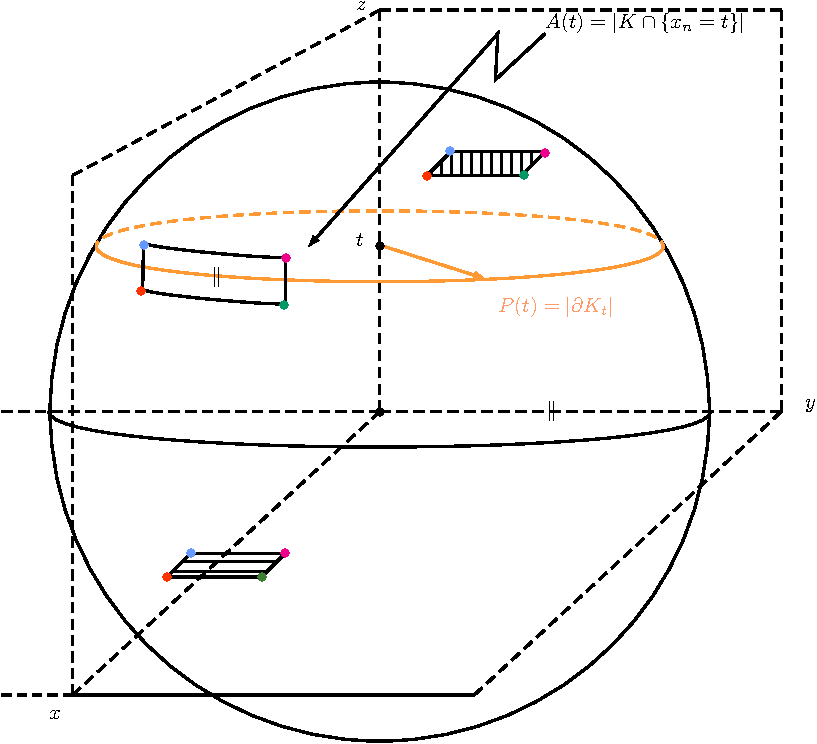
\includegraphics[scale=.9]{images/proof.pdf}
\caption{Depiction of the situation as described by G. Lawlor. Pay attention to the projection on the tangential horizontal subspace denoted by $\|$.}
\end{figure}
\end{proof}
\begin{remark} The above method may provide a more suitable approach of a proof for undergraduate students, however there is still work to be done by turning the arguments into rigorous statements applicable to multivariable calculus. 
\end{remark}
\newpage
We require the following auxiliary lemma
\begin{lemma} There exists a differentiable function $h: [t_1,t_2] \to [-r,r]$, where $r$ is the (fixed radius) of $B_n$ such that $|B_n|=|K|$, which satisfies
\begin{align*}
\int_{- \infty}^\tau A(t)dt = \frac{|B_{n-1}|}{r^{n-1}} \int_{-r}^{h( \tau)} (r^2-s^2)^{\frac{n-1}{2}} ds. 
\end{align*}
\end{lemma}
\begin{remark} Informally speaking, $h$ matches the volume up to height $h( \tau) \in [-r,r]$  of the ball $B_n$ with radius $r$ with the volume of $K$ up to height $\tau$. 
\end{remark}
\begin{proof}
By our choice of $r$, we have 
\begin{align*}
\int_{- \infty}^\infty A(t)dt = \int_{t_1}^{t_2} A(t)dt = |K|=|B_n| = \frac{|B_{n-1}|}{r^{n-1}} \int_{-r}^r (r^2-s^2)^\frac{n-1}{2}ds.
\end{align*}
This can be verified by seeing that 
\begin{align*}
|B_n| = \frac{\pi^\frac{n}{2}}{\Gamma \left( \frac{n}{2}+1\right)}r^n, \ |B_{n-1}| = \frac{\pi^\frac{n-1}{2}}{\Gamma \left( \frac{n-1}{2}+1\right)}r^{n-1} =\frac{\pi^\frac{n-1}{2}}{\Gamma \left( \frac{n+1}{2}\right)}r^{n-1} 
\end{align*}
and
\begin{align*}
\int_{-r}^r (r^2-s^2)^\frac{n-1}{2}ds = \frac{\sqrt{\pi}  \Gamma\left( \frac{n+1}{2}\right)}{\Gamma \left( \frac{n}{2}+1\right)}r^n.
\end{align*}
Thus we establish that 
\begin{align*}
|B_{n-1}| \int_{-r}^r (r^2-s^2)^\frac{n-1}{2}ds &= \frac{\pi^\frac{n-1}{2}}{\Gamma \left( \frac{n+1}{2}\right)}r^{n-1} \frac{\sqrt{\pi} \Gamma\left( \frac{n+1}{2}\right)}{\Gamma \left( \frac{n}{2}+1\right)}r^n \\
&= r^{n-1} \frac{\pi^\frac{n}{2}}{\Gamma \left( \frac{n}{2}+1\right)}r^n = r^{n-1}|B_n|.
\end{align*}
Now consider $g:[t_1,t_2] \to \text{Image}(g) \subset \mathbb{R}_+$ and $f:[-r,r] \to \text{Image}(f) \subset \mathbb{R}_+$ given by \begin{align*}
g(t):= \int_{t_1}^t A(s)ds, \text{ and } f(t):= \frac{|B_{n-1}|}{r^{n-1}} \int_{-r}^t (r^2-s^2)^\frac{n-1}{2}ds.
\end{align*}
Then both $g$ and $f$ are continuously differentiable functions, strictly monotone increasing and thus bijective. Moreover, since $g(t_1)=f(-r)$ and $g(t_2)=f(r)$ they must have the same image. Hence $f,g$ are both bijections on the same set, say Image. By the inverse function theorem $f^{-1}: \text{Image} \to [-r,r]$ is again continuously differentiable, hence so is $h:=f^{-1} \circ g : [t_1,t_2] \to [-r,r]$ and certainly we have 
\begin{align*}
f(h(t))=f(f^{-1} \circ g (t)) = f(f^{-1}(g(t))=g(t).
\end{align*}
\end{proof}
By differentiation we immediately get:
\begin{corollary} \label{C1} For all $t \in [t_1,t_2]$ we have
\begin{align*}
A(t) = \frac{|B_{n-1}|}{r^{n-1}} (r^2-h(t)^2)^\frac{n-1}{2} h'(t).
\end{align*}
\end{corollary}
We are now in a good position to give a proof of Theorem \ref{T1Ref}. The proof we give follows the arguments presented by Gary Lawlor in his 2010 print \textit{An elementary isoperimetric proof in $n$-space} which is in fact a proof by induction over the dimension $n$ of $\mathbb{R}^n$. 
\begin{proof}[Proof of Theorem \ref{T1Ref}] We proceed by induction over the dimension $n$ of $\mathbb{R}^n$. For $n=1$, we've already established the claim in remark \ref{R1}.1. Moving up a dimension, let us assume that
\begin{align*}
\frac{(n-1)|B_{n-1}|}{r'} \leq | \partial K|
\end{align*}
where $B_{n-1}$ is a $(n-1)$-dimensional sphere of radius $r'$ such that $|B_{n-1}|=|K|= \lambda_{n-1}(K)$ for a domain $K \subset \mathbb{R}^{n-1}$. 
As already discussed in remark \ref{R1}.3. we can choose $r$ such that $|B_n|=|K|$ and thus it suffices to show that for a domain $K  \subset \mathbb{R}^n$
\begin{align*}
| \partial B_n| \leq | \partial K|.
\end{align*}
Corollary \ref{C1} guarantees the existence of a differentiable function $h: \mathbb{R} \to [-r,r]$ such that 
\begin{align*}
A(t) = \frac{|B_{n-1}|}{r^{n-1}} (r^2-h(t)^2)^\frac{n-1}{2} h'(t).
\end{align*}
Defining $f(t):= h'(t)^{-\frac{1}{n-1}}$ establishes that
\begin{align*}
f(t)^{n-1}h'(t)=1.
\end{align*}
Moreover, both $f$ and $h'$ are nonnegative as is easily seen by the formulas above and thus, by the AM-GM inequality, we get
\begin{align*}
(n-1)f(t)+h'(t) \geq n \sqrt[n]{f(t)^{n-1}h'(t)}=n.
\end{align*}
Next, we apply the Cauchy-Schwarz inequality $( \langle u ,v \rangle \leq | \langle u,v \rangle| \leq \|u\| \|v\|$) to the vectors
\begin{align*}
u = \binom{P(t)}{A'(t)}, \ v= \binom{ \sqrt{r^2-h(t)^2}}{-h(t)}
\end{align*}
to establish 
\begin{align*}
 \langle u, v \rangle= P(t) \sqrt{r^2-h(t)^2} - A'(t)h(t) \leq \|v\| \|u\| = r \sqrt{P(t)^2+A'(t)^2}
\end{align*}
\newpage
Thus 
\begin{align} \label{eq1}
\sqrt{P(t)^2 +A'(t)^2} \geq  \frac{1}{r}P(t)\sqrt{r^2-h(t)^2} - \frac{1}{r}A'(t)h(t) 
\end{align}
Let us recall our induction hypothesis, for any surface in $\mathbb{R}^{n-1}$ which has the same volume as round sphere $B_{n-1}$ of radius $r$, the surface area $S$ satisfies 
\begin{align*}
S \geq \frac{(n-1)|B_{n-1}|}{r}.
\end{align*}
Hence if we apply this induction hypothesis on $P(t)$ we get 
\begin{align*}
P(t) \geq \frac{(n-1) |\widetilde{B}_{n-1}|}{\widetilde{r}}
\end{align*}
where the radius $\widetilde{r}$ of $\widetilde{B}_{n-1}$ has to be chosen such that $|\widetilde{B}_{n-1}| = A(t)$. By corollary \ref{C1} we have  
\begin{align*}
A(t)  = \frac{|B_{n-1}|}{r^{n-1}} (r^2-h(t)^2)^\frac{n-1}{2} h'(t) \overset{!}= |\widetilde{B}_{n-1}| 
\end{align*}
which allows us (by plugging in the closed formulas for $|B_{n-1}|$ and $|\widetilde{B}_{n-1}|$) to solve for $\widetilde{r}$ as
\begin{align*}
\widetilde{r} = \sqrt{r^2-h(t)^2}h'(t)^\frac{1}{n-1} = \frac{\sqrt{r^2-h(t)^2}}{f(t)}.
\end{align*}
Bringing this together we have shown that 
\begin{align}
P(t) \geq \frac{(n-1)A(t)f(t)}{\sqrt{r^2-h(t)^2}}. \label{eq2}
\end{align}
Using (\ref{eq2}) to further estimate (\ref{eq1}) we get 
\begin{align} \label{eq3}
\sqrt{P(t)^2 +A'(t)^2} &\geq  \frac{1}{r} \left[ (n-1)A(t)f(t) - A'(t)h(t) \right] \notag \\
& \geq \frac{1}{r}\left[ A(t)(n-h'(t))- A'(t)h(t) \right] \notag \\
&= \frac{1}{r} \left[ nA(t)- (h'(t)A(t)+A'(t)h(t)) \right] \notag \\
&= \frac{1}{r} \left[ nA(t) - (h(t)A(t))'\right]
\end{align}
\newpage
We now use (\ref{eq3}) to wrap up the proof as follows: applying Proposition \ref{P1}
\begin{align*}
| \partial K| &= \int_{t_1}^{t_2} \sqrt{P(t)^2+A'(t)^2}dt \geq \int_{t_1}^{t_2} \frac{1}{r}[nA(t)-(h(t)A(t))' ] dt \\
&= \frac{1}{r}n \int_{t_1}^{t_2} A(t)dt - \frac{1}{r} \int_{t_1}^{t_2} (h(t)A(t))'dt  \\
&= \frac{n}{r} |K| = \frac{n}{r}|B_n| = | \partial B_n|.
\end{align*}
Where we used that $A(t_1)=A(t_2)=0$ and its easy to verify with the help of the closed formulas that $\frac{n}{r}|B_n|= | \partial B_n|$. This concludes the proof. 
\end{proof}
\end{document}
